\documentclass[a4paper,12pt]{article}
\usepackage[T2A]{fontenc}
\usepackage[utf8]{inputenc}
\usepackage[english, russian]{babel}
\usepackage{minted}
\usepackage{verbatim}
\usepackage{graphicx}
\usepackage{caption}
\usepackage{subcaption}
\usepackage[left=2.5cm,right=2.5cm,top=2cm,bottom=2cm]{geometry}

\newenvironment{longlisting}{\captionsetup{type=listing}}{}

\newenvironment{pseudolisting}
 {\begin{minipage}{\linewidth}\vspace*{\topsep}}
 {\vspace*{\topsep}\end{minipage}}

\begin{document}

\begin{titlepage}
  \begin{center}
    \large
     
    \textbf{}

 

    
    \vfill
     
     
   
    \vfill
 
    \textsc{Лаборатная работа №2, вариант №23}\\[5mm]
     
    {\LARGE РЕШЕНИЕ СИСТЕМ ЛИНЕЙНЫХ АЛГЕБРАИЧЕСКИХ УРАВНЕНИЙ
ПРЯМЫМИ МЕТОДАМИ. ТЕОРИЯ ВОЗМУЩЕНИЙ\\[2mm]
    }
    \textsc{Задания: 3.1.23, 3.3.6, 3.8.5}\\[5mm]
  \bigskip
     
    
\end{center}
\vfill
 

 
\hfill\begin{flushright}
  \textbf{Студент:}\\
  Паршина Софья Романовна \\
  3 курс, группа БПМ213
\end{flushright}%
\vfill

\end{titlepage}


\tableofcontents

\section{Погрешность решения при изменение правой части(3.1.23)}
\subsection{Формулировка задачи}
\begin{figure}[H]
\centering
  \includegraphics[width=\linewidth]{1 номер.png}
\end{figure}

$$N = 23, n = 5$$
$$ c_ij=0.1*N*i*j $$
$$a_ij=\frac{11.7}{(1+c)^7}$$
\subsection{Код на Python}

\begin{longlisting}
\inputminted{python}{cond.py}
\end{longlisting}

\subsection{Результат работы программы}
\begin{longlisting}
\verbatiminput{cond.txt}
\end{longlisting}
Практическая погрешность была взята $\Delta = 0.1$, a $\delta{(x^m)} = 0.0076...$ -> теоретическая погрешность решения $x^m$ меньше.
Из результатов работы программы можно увидеть, что формула для теоретической оценки верна, так как правая часть существенно больше левой. 


\subsection{График погрешности в зависимости от возмущения правой части}
\begin{figure}[H]
\centering
\begin{subfigure}{.5\textwidth}
  \centering
  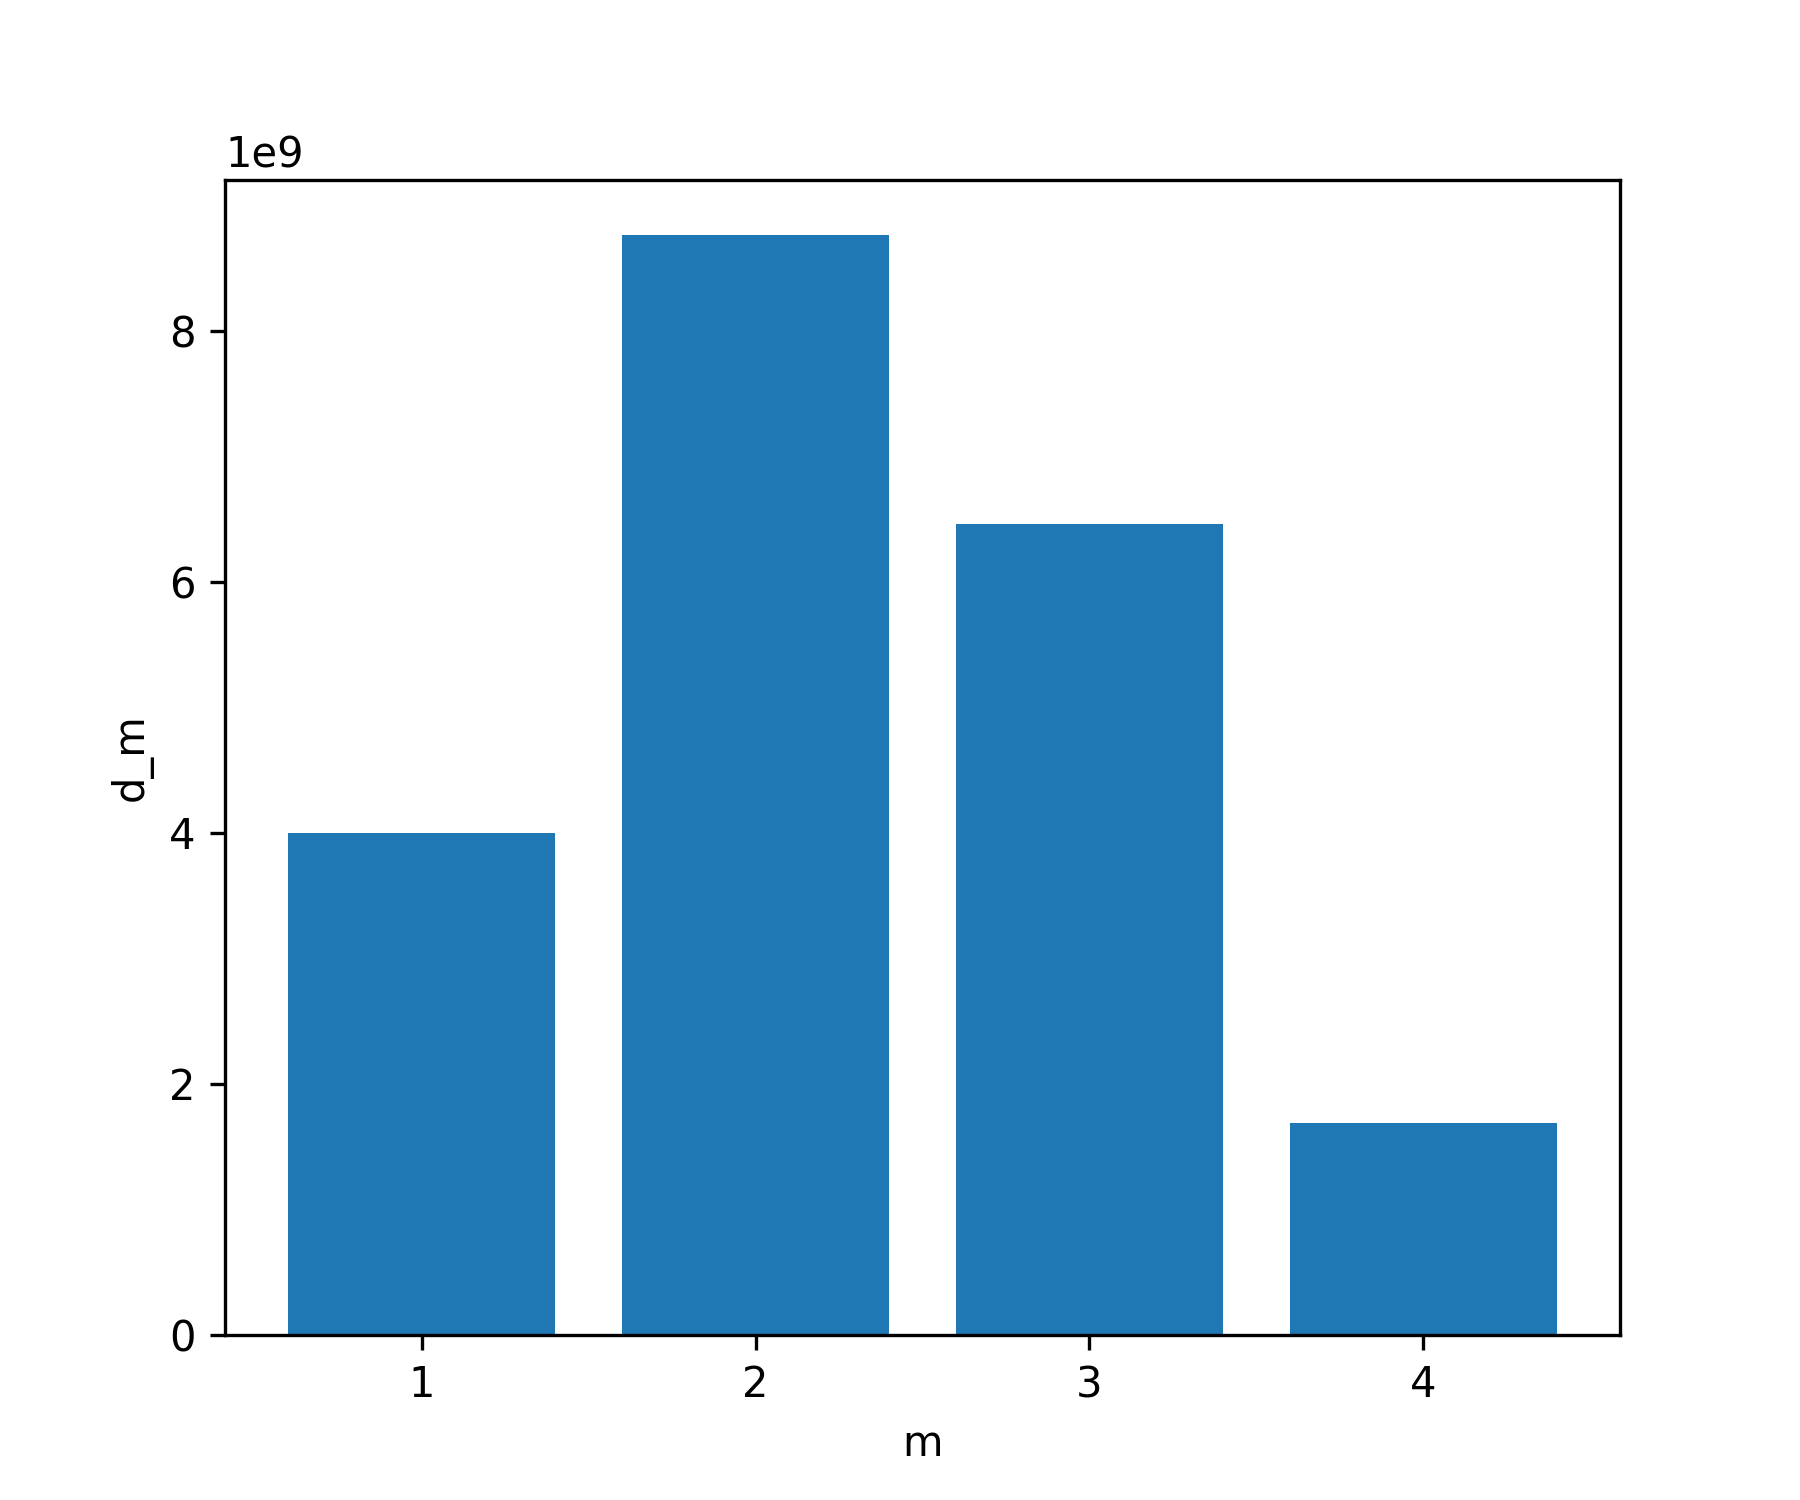
\includegraphics[width=\linewidth]{cond_precision.png}
  \label{fig:sub1}
\end{subfigure}%
\caption{Наибольшее влияние на погрешность решения вносит компонента $b_m$, $m=5$}
\label{fig:test}
\end{figure}

\section{Число обусловенности матрицы(3.3.6)}
\subsection{Формулировка задачи}
\begin{figure}[H]
\centering
  \includegraphics[width=\linewidth]{3_1.png}
  \includegraphics[width=\linewidth]{3_2.png}
\end{figure}
Матрица А = 
\left[
\begin{array}{rrrr}
611 & 196 & -192 & 407\\
196 & 899 & 113 & -192\\
-192 & 113 & 899 & 196\\
407 & -192 & 196 & 611
\end{array}
\right]
\subsection{Код на Python}
\begin{longlisting}
\inputminted{python}{cond_2.0.py}
\end{longlisting}

\subsection{Результат работы программы}
\begin{longlisting}
\verbatiminput{cond_2.0.txt}
\end{longlisting}

Число обсуловленности, полученное экспериментально, близко к числу, полученному с помощью встроенной функции. Погрешность накапливается по ходу вычислений, поэтому в результатах есть различие.

\section{Метод Гаусса - схема полного выбора(3.8.5)}
\subsection{Формулировка задачи}
\begin{figure}[H]
\centering
  \includegraphics[width=\linewidth]{8.jpg}
  \includegraphics[width=\linewidth]{8_1.jpg}
\end{figure}
$$M=5, n=100, b_i=| x - \frac{n}{10}|*i*\sin{(x)}$$
\subsection{Код на Python}

\begin{longlisting}
\inputminted{python}{gauss.py}
\end{longlisting}

\subsection{Результат работы программы}
Было взято 50 точек х в интервале от [-5, 5], равномерно распределённых.
Решение реализованное и решение из библиотеки Python cовпадаеn - это видно из графиков.
\subsection{График реализованного метода Гаусса $y(x)$ и встроенного метода Гаусса $orig(x)$}
\begin{figure}[H]
\centering
\begin{subfigure}{.5\textwidth}
  \centering
  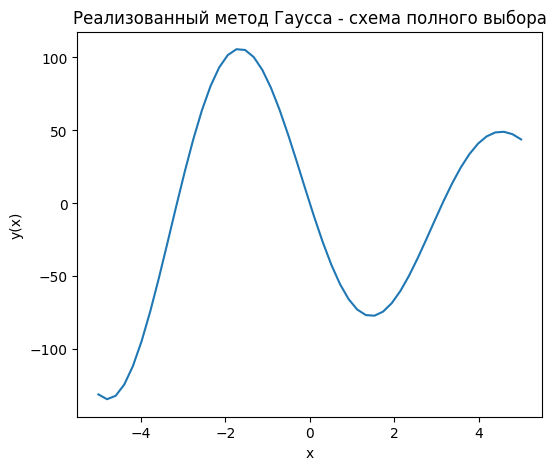
\includegraphics[width=\linewidth]{graphic.png}
  \includegraphics[width=\linewidth]{orig_graphic.png}
  \label{fig:sub1}
\end{subfigure}%
\label{fig:test}
\end{figure}

\end{document}
